\chapter{Vektorové datové modely}
\label{chap:vektorovedatovemodely}
	Následující odstavce byly čerpány z publikací \cite{kolar2003geograficke,tucek1997geograficke,vesely2007thesis}. K uchování prostorových dat v GIS jsou používané dva základní typy, a to vektorová a rastrová data. Rastrová data se hojně využívají pro popis spojitého jevu, například nadmořské výšky, nebo pro fotoplány. Každý pixel obsahuje jednu číselnou hodnotu. Jeden rastrový obraz může obsahovat i více vrstev, pak může být fotoplán vyjádřen hodnotami barev RGB, zatímco nadmořská výška bude pravděpodobně vyjádřena jednou číselnou hodnotou.
	
	Druhým typem je vektorové vyjádření. Klasický vektor, tak jak ho známe z matematiky, je charakterizován velikostí a směrem. Lze ho ovšem vyjádřit i dvěma body, čehož využíváme ve vektorové grafice. Odtud je tedy zřejmé, proč vektorová grafika nese toto označení. V GIS se využívají tři základní geometrické útvary. Těmi jsou body, linie a polygony. Tyto základní typy pak slouží pro popis objektů v krajině.
	
	\textbf{Bod} je nejjednodušší geometrický prvek. Nese v sobě informaci o poloze, vyjádřenou souřadnicemi $X$, $Y$, případně $Z$.
	
	\textbf{Linie} je vyjádřena posloupností souřadnic. Linie začíná a končí v uzlech, její mezilehlé body se nazývají vertexy. Podle topologických pravidel by linie v jedné vrstvě měly být napojeny pouze přes uzly. Tento topologický koncept se nazývá \textit{konektivita}.
	
	\textbf{Polygon} je vyjádření plochy. Je vyjádřen obdobně jako linie posloupností souřadnic, ovšem počáteční a koncový uzel jsou totožné. To vychází z druhého konceptu topologie, který se nazývá \textit{definice plochy}.
	
	Každý vektorový objekt může kromě geometrické informace obsahovat také různé atributy. Tyto atributy jsou propojeny s objektem pomocí jeho identifikátoru. Li\-ni\-o\-vý prvek vyjadřující pozemní komunikaci proto může obsahovat atributy jako je číslo silnice, maximální povolená rychlost a mnoho dalších, což je značná výhoda oproti rastrovému vyjádření, kde by bylo toto velmi obtížné.
	
\section{Špagetový model}
	Tento model je velice jednoduchý, každý objekt je uložen jako jeden záznam v datové tabulce. Tato tabulka obsahuje identifikátor prvku a jeho souřadnice. Tento model neukládá žádné prostorové vztahy. Je tedy velice jednoduché přidání či odebrání objektu. Pouze smažeme či přidáme řádek do příslušné tabulky. Tento model je vhodný pro vizualizaci či přenos dat. Nevýhodou je, že společné hranice polygonů jsou v tomto modelu uloženy 2x, pro každý polygon zvlášť. Problém nastává také při některých geometrických analýzách. Jelikož nám nejsou známé žádné prostorové vztahy, musíme například pro zjištění sousedních polygonů projít všechny záznamy v tabulce. Tyto chybějící prostorové vztahy musí být často dopočteny a po provedení analýzy je opět ztrácíme. Pokud tedy nad většími daty chceme provádět často rozsáhlejší prostorové analýzy, tento model není příliš vhodný pro jejich uchovávání.
	
\section{Topologické modely}
	Jak z názvu vyplývá, topologické modely uchovávají informace o topologii. Tedy o prostorových vztazích objektů mezi sebou. Data uložená v topologickém modelu jsou velkou výhodou pro geometrické analýzy, které díky struktuře dat mají mnohé vztahy předpočítané a uložené v datové struktuře. Existuje mnoho způsobů pro uchování topologického modelu. Jako příklad topologického modelu může být formát \textit{GDF/DIME} vyvinutý a používaný v sedmdesátých a osmdesátých letech v USA~\cite{walford2002geographical}.

\subsubsection{Topologie bodů}
	Topologie bodů je velice jednoduchá a v podstatě koresponduje s uchováním dat ve špagetovém modelu. Jelikož jsou body jeden na druhém nezávislé, nejsou zde uloženy žádné zvláštní topologické vztahy. Jediné, co je o bodech uchováváno, je jejich identifikátor, přes který lze bod propojit se souřadnicemi.
	
\subsubsection{Topologie linií}
	Pro linie platí pravidlo, že každé dvě linie mohou sdílet pouze uzly, tedy koncové body. Každá část linie je uložena s odkazem na uzly linie. Struktura dále ukládá informace o pravém a levém polygonu vzhledem ke směru linie, pokud takovýto polygon existuje.

\subsubsection{Topologie polygonů}
	Pro každý polygon je definováno odkazy na linie, které ho ohraničují. Výhoda v tomto modelu je, že společné linie polygonů jsou uloženy pouze jednou.
	
Ze struktury dat je vidět, že velice snadno zjistíme například sousední polygony k námi vybranému polygonu. Učinit tak můžeme bez jakéhokoliv přístupu k souřadnicím a geometrickým výpočtům, narozdíl od špagetového modelu. To může ušetřit mnoho času při prostorových analýzách.

\begin{figure}[h]
  \centering
  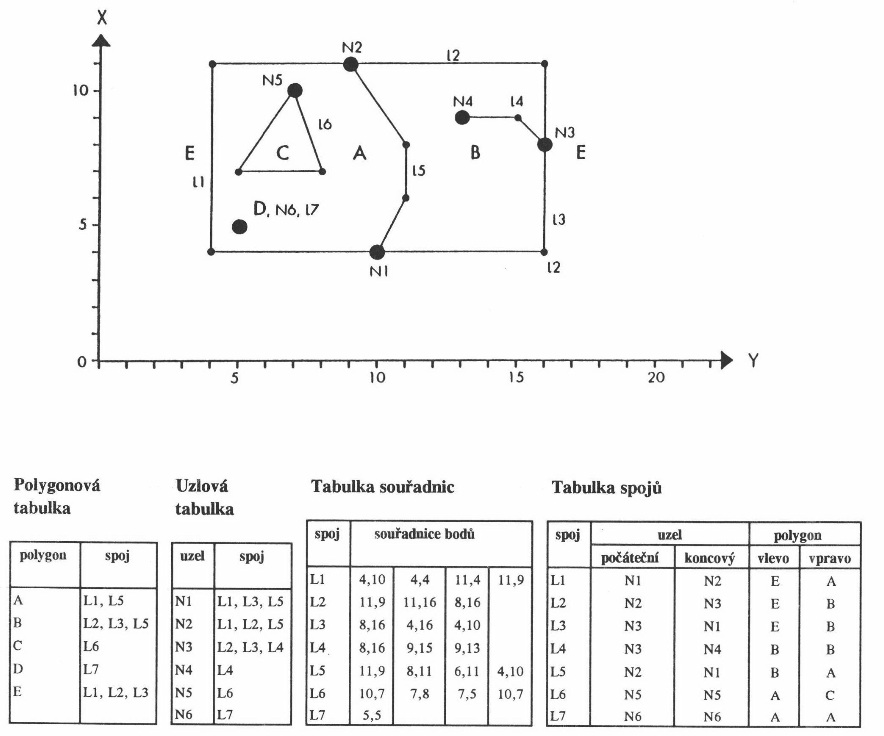
\includegraphics[width=10cm]{./pictures/3/topo_model.png}
  \caption{Ukázka topologického modelu (převzato z \cite{kolar2003geograficke})}
  \label{fig:3-time_complexity}
\end{figure}
